\chapter[Kovariante Formulierung]{Kovariante Formulierung der Elektrodynamik}

\section{Raum-Zeit-Begriff und Lorentz-Transformation}

Bevor wir zur eigentlichen Elektrodynamik kommen, müssen zunächst ein paar essentielle Begriffe eingeführt werden:\\

Ein \textbf{Bezugssystem} ist ein Koordinatensystem zu Bestimmung der räumlichen Lage $\vec{r}$ eines Teilchens, zusammen mit einer Uhr für die Zeit $t$. Es stellt sich heraus, dass Ort und Zeit relativ, also abhängig vom Bezugssystem sind.\\

Ein \textbf{Inertialsystem} ist ein Bezugssystem, in dem ein sich frei bewegender Körper eine konstante Geschwindigkeit besitzt.\\

Das \textbf{Relativitätsprinzip} besagt, dass die Naturgesetze in allen Inertialsystem diesselbe Form haben. Wir werden in diesem Zusammenhang später auf Begriffe wie "`Invarianz"' oder "`Kovarianz"' stoßen.\\ 

\begin{enumerate}
\item \textbf{\textsc{ Galilei}}\\

Damals ging man vom Relativitätsprinzip und von der instantanen Ausbreitung von Wirkungen aus. Demnach hingen Kräfte nur von der aktuellen Position der Teilchen ab.
\newpage
Der Wechsel zwischen zwei mit der Relativgeschwindigkeit $\vec{v}$ zueinander bewegten Inertialsystemen wird durch die \textsc{Galilei}-Transformation beschrieben. 
\begin{equation*}
\vec{r}'=\vec{r}+\vec{v}t
\end{equation*}
Wichtig ist dabei, dass $t=t'$ gilt.\\

\item \textbf{\textsc{ Einstein}}\\

Es wird neben Relativitätsprinzip zusätzlich noch der Ausbreitung von Wirkungen mit Lichtgeschwindigkeit ausgegangen. Diese hat in jedem Intertialsystem denselben Wert! \\
Der Übergang zwischen zwei System wird hier durch die \textsc{Lorentz}-Transformation realisiert.\\ 
\end{enumerate}

Zur eleganten Formulierung der Speziellen Relativitätstheorie (es werden nur Intertialsysteme betrachtet) führt man den \textbf{\textsc{Minkowski}-Raum} ein, der neben den drei Raumdimensionen noch die Zeit als eigene Dimension enthält. \\
Punkte in diesem Raum sind natürlich keine \emph{Orte}, sondern \emph{Ereignisse}.\\
Die Elemente dieses Raums bezeichnen wir als \textbf{Vierervektoren} und verwenden die Schreibweise
\begin{equation*}
x^\mu = (x^0,x^1,x^2,x^3)=(ct,x,y,z).
\end{equation*}
In der Speziellen Relativitätstheorie (SRT) ist es üblich, für Indizes, die die Werte 0 bis 3 annehmen, griechische Buchstaben zu verwenden.\\

Abstände zwischen zwei Punkten (Ereignissen) werden nach
\begin{equation*}
\mathrm{d}s^2 = c^2\mathrm{d}t^2 -\mathrm{d}x^2 - \mathrm{d}y^2 - \mathrm{d}z^2 
\end{equation*}
definiert. Das lässt sich alternativ auch unter Verwendung des metrischen Tensors $g_{\mu\nu}$ ausdrücken.
\begin{empheq}[box=\highlightbox]{equation*}
\mathrm{d}s^2 = g_{\mu\nu}\mathrm{d}x^\mu\mathrm{d}x^\nu \qquad \text{mit}\ g_{\mu\nu}=\begin{pmatrix}
1 & 0& 0 & 0 \\
0 &-1& 0 & 0\\
0 & 0 & -1 & 0 \\
0 & 0 & 0 & -1 \\
\end{pmatrix}
\end{empheq}
\emph{Bemerkung: Hier wird die \textsc{Einstein}sche Summenkonvention verwendet. Über Indizes, die einmal oben und einmal unten auftauchen, wird summiert!}\\

Für die Lichtausbreitung gilt $\mathrm{d}s=0$ in allen Intertialsystemen. \\
Betrachten wir nun zwei Inertialsysteme $k$ und $k'$, die sich mit konstanter Geschwindigkeit $\vec{v}$ relativ zueinander bewegen und zwei Ereignisse mit den infinitessimalen Abständen $\mathrm{d}s$ und $\mathrm{d}s'$. \\
Wir zeigen nun, dass eine \textsc{Lorentz}-Transformation immer $\mathrm{d}s=\mathrm{d}s'$ gewährleistet. \\

Aus der Konstanz von $c$ folgt, dass $\mathrm{d}s$ genau dann Null sein muss, wenn $\mathrm{d}s'$ auch Null ist. Der Zusammenhang zwischen den beiden muss also linear sein!\\
Der der Raum homogen und isotrop ist, kann dieser Zusammenhang nicht von den Orten der Bezugssysteme, sondern nur vom Betrag der Relativgeschwindigkeit $|\vec{v}|$ abhängen. Jetzt nehmen wir uns drei Inertialsysteme $k_1,\ k_2$ und $k_3$. 
\begin{align*}
\mathrm{d}s_1^2 &= a(v_{12})\mathrm{d}s_2^2\\
\mathrm{d}s_2^2&=a(v_{23})\mathrm{d}_3^2\\
\mathrm{d}s_1^2 &=a(v_{13})\mathrm{d}s_3^2
\end{align*}
Das heißt
\begin{equation*}
a(v_{23})=\frac{a(v_{13})}{a(v_{12})}.
\end{equation*}
$v_{23}$ muss aber von $v_{12}$, $v_{13}$ und dem Winkel zwischen den beiden abhängen. Deshalb müssen alle $a=1$ sein. Der Viererabstand $\mathrm{d}s$ ist also invariant unter \textsc{Lorentz}-Transformation.\\

Für \textbf{zeitartige Abstände} ($\mathrm{d}s^2>0$) existiert für zwei Ereignisse ein Intertialsystem $k'$, in dem beide am gleichen Ort stattfinden, denn
\begin{equation*}
c^2\mathrm{d}t'^2 = c^2\mathrm{d}t^2 - \mathrm{d}\vec{r}^2 \qquad \Rightarrow \mathrm{d}\vec{r}'^2 = 0.
\end{equation*} 

Für \textbf{raumartige Abstände} ($\mathrm{d}s^2<0$) existiert für zwei Ereignisse ein Inertialsystem, in dem beide gleichzeitig stattfinden, denn
\begin{equation*}
-\mathrm{d}\vec{r}^2 =c^2\mathrm{d}t^2-\mathrm{d}\vec{r}^2 \qquad \Rightarrow \mathrm{d}t'^2 =0.
\end{equation*}
Da $\mathrm{d}s^2$ invariant unter \textsc{Lorentz}-Transformation ist, sind raum- und zeitartige Abstände absolut.\\

Als \textbf{Eigenzeit} eines Beobachters oder Teilchens bezeichnet man die Zeit, die von der Uhr angezeigt wird, die sich mit ihm mitbewegt. Dabei kann der Beobachter beliebig bewegt (sogar beschleunigt) sein. Eine Uhr mit einem fest verbundenen Koordinatensystem, das nicht unbedingt ein Inertialsystem sein muss, definiert ihr \textbf{momentanes Inertialsystem}.
\begin{align*}
\mathrm{d}s^2 &= c^2\mathrm{d}t^2 - \mathrm{d}\vec{r}^2 = c\mathrm{d}\tau^2-0\\
\mathrm{d}\tau^2 &= \mathrm{d}t^2\left(1-\frac{1}{c^2}\left(\diff{\vec{r}}{t}\right)^2\right)=\mathrm{d}t^2\left(1-\frac{v^2}{c^2}\right)\\
%\Rightarrow \mathrm{d}t &= \frac{\mathrm{d}\tau}{\sqrt{1-\frac{v^2}{c^2}}}\geq \mathrm{d}\tau
\end{align*}
Die letzte Zeile bezeichnet den Effekt der \textbf{Zeitdilatation}.\\ \linebreak

\textbf{\textsc{Lorentz}-Transformation}\\

Es handelt sich dabei um eine Transformation der Koordinaten $(t,\vec{r})$ eines Ereignisses im Inertialsystem $k$ in die Koordinaten $(t',\vec{r}')$ desselben Ereignisses in $k'$. Die Prämisse dabei ist, dass die Transformation aufgrund der Homogenität von Raum und Zeit linear sein muss und $\mathrm{d}s^2$ konstant sein muss. \\
Wir betrachten o.B.d.A. den Fall $\vec{e}_x\parallel\vec{e}_x'\parallel\vec{v}$. Der allgemeine Ansatz ist
\begin{align*}
t'&=a(x-wt)\\
x'&=a(x-ut)\\
y'&=y\\
z'&=z
\end{align*}
Natürlich muss $u=v=|\vec{v}|$ sein. Ebenso müssen $a$ und $b$ denselben Wert haben. Wir fordern
\begin{align*}
\mathrm{d}s^2 &=\mathrm{d}s'^2\\
c^2\mathrm{d}t^2-\mathrm{d}x^2 &=a^2c^2(\mathrm{d}t+w\mathrm{d}x)^2 - a^2(\mathrm{d}x-v\mathrm{d}t)^2
\end{align*}
Ein Koeffizientenvergleich liefert 
\begin{align*}
a&=\frac{1}{\sqrt{1-\frac{v^2}{c^2}}} & w&=-\frac{v}{c^2}.
\end{align*}
Wir kürzen $(1-\frac{v^2}{c^2})^{\frac{1}{2}}$ mit $\gamma$ ab und erhalten die spezielle (nicht kommutative) \textsc{Lorentz}-Transformation
\begin{empheq}[box=\highlightbox]{align*}
x'&=\gamma(x-vt) & x &=\gamma(x'+vt')\\
t'&=\gamma\left(t-\frac{v}{c^2}x\right) & t &=\gamma\left(t'+\frac{v}{c^2}x'\right)\\
y &=y'   & z' &=z
\end{empheq}

Eine Folgerung der \textsc{Lorentz}-Transformation ist die \textbf{Längenkontraktion}:\\
Ist ein Objekt in $k'$ in Ruhe und habe dort die Länge $l_0$. In $k$ hat es jedoch die Länge
\begin{equation*}
l = \frac{l_0}{\gamma} < l_0.
\end{equation*}
Geschwindigkeiten transformieren nach
\begin{align*}
u_x' &= \diff{x'}{t'}=\frac{\mathrm{d}x-v\mathrm{d}t}{\mathrm{d}-\frac{v}{c^2}\mathrm{d}x}=\frac{u_x-v}{1-\frac{vu_x}{c^2}}\\
u_y' &=\frac{u_y\sqrt{1-\frac{v^2}{c^2}}}{1-\frac{vu_x}{c^2}}
\end{align*}
beziehungweise
\begin{align*}
u_\parallel' &=\frac{u_\parallel-v}{1-\frac{\vec{v}\vec{u}}{c^2}}\\
u_\perp' &= \frac{u_\perp\sqrt{1-\frac{v^2}{c^2}}}{1-\frac{\vec{v}\vec{u}}{c^2}}
\end{align*}
Im Grenzfall kleiner Geschwindigkeiten $\vec{v}$ geht die \textsc{Lorentz}-Transformation in eine \textsc{Galilei}-Transformation über.

\section{Vierergrößen und Kovarianz}

Im dreidimensionalen Raum transformieren sich die Komponenten eines Vektors bei Drehung.
\begin{equation*}
\vec{r}'=\tens{R}\vec{r} \qquad (\det\tens{R}=\pm 1)
\end{equation*}
Skalare (z.B. $\vec{r}^2=x^2+y^2+z^2$, $\vec{A}\cdot\vec{B}=A_xB_x+A_yB_y+A_zB_z$) bleiben unter Drehung invariant. Im vierdimensionalen \textsc{Minkoswki}-Raum bleibt das im Prinzip erhalten. Aufgrund der Abstandsdefinition handelt es sich jedoch um eine nicht-euklidische Metrik.\\
Wir definieren
\begin{align*}
x^\mu &= (ct,x,y,z)=(x^0,x^1,x^2,x^3)=(ct,\vec{r})=(ct,\vec{x})\\
\mathrm{d}x^\mu & = (c\mathrm{d}t,\mathrm{d}\vec{r})
\end{align*}
Die Transformationseigenschaften von $x^\mu$ und $\mathrm{d}x^\mu$ sind bekannt. Eine \textsc{Lorentz}-Transformation entspricht einer Drehung im \textsc{Minkowski}-Raum.\\

\textbf{Kontravariante Vektoren}

\begin{equation*}
A^\mu = (A^0,A^1,A^2,A^3)
\end{equation*}
Sie transformieren sich wie $x^\mu$, das heißt
\begin{equation*}
A'^\mu =\pdiff{x'^\mu}{x^\nu}A^\nu
\end{equation*}
\ \\

\textbf{Kovariante Vektoren}
\begin{equation*}
A_\mu=(A_0,A_1,A_2,A_3)
\end{equation*}
mit
\begin{equation*}
A_\mu'=\pdiff{x^\nu}{x'^\mu}A_\nu
\end{equation*}

Aus diesen Transformationseigenschaften folgt, wie wir später sehen werden,
\begin{equation*}
A_\nu = g_{\mu\nu}A^\mu.
\end{equation*}

\textbf{Skalarprodukt}\\

Das Skalarprodukt zwischen zwei Vierervektoren definiert man durch
\begin{equation*}
A\cdot B = A_\mu\cdot B^\mu = g_{\mu\nu}A^\mu B^\nu = A^\mu B_\mu.
\end{equation*}
Es ist invariant unter \textsc{Lorentz}-Transformation, denn
\begin{equation*}
A'\cdot B' = \pdiff{x^\nu}{x'^\mu}\pdiff{x'^\mu}{x^\kappa} A_\mu B^\kappa = \pdiff{x^\nu}{x^\kappa}B^\kappa A_\nu = A\cdot B.
\end{equation*}

\textbf{Indexkontraktion mit $g$}

\begin{equation*}
g_{\mu\nu}=g^{\mu\nu}=\begin{pmatrix}
1 & 0& 0 & 0 \\
0 &-1& 0 & 0\\
0 & 0 & -1 & 0 \\
0 & 0 & 0 & -1 \\
\end{pmatrix}, \qquad g_{\mu\nu}g^{\nu\kappa}=\delta_\mu^\kappa
\end{equation*}
\begin{equation*}
\mathrm{d}s^2 = g_{\mu\nu}\mathrm{d}x^\mu\mathrm{d}x^\nu=\mathrm{d}x_\nu\mathrm{d}x^\mu
\end{equation*}

\newpage
\textbf{Ableitungen im \textsc{Minkowski}-Raum}\\

Beim Differenzieren ist darauf zu achten, dass die Ableitung nach einem kontravarianten selbst wieder einen kovarianten Vektor liefert. Wir definieren
\begin{align*}
\partial^\alpha &= \pdiff{}{x_\alpha}=\left(\pdiff{}{x^0},-\nabla\right)\\
\partial_\alpha &= \pdiff{}{x^\alpha}=\left(\pdiff{}{x_0},\nabla\right).
\end{align*}
Diese Schreibweisen verdeutlichen, dass sowohl die Viererdivergenz, also auch der Wellenoperator invariant sind.
\begin{align*}
\partial_\alpha A^\alpha &= \partial^\alpha A_\alpha =\pdiff{A^0}{x^0}+\div\vec{A}\\
\partial_\alpha\partial^\alpha&=\partial^\alpha\partial_\alpha = \left(\pdiff{}{x^0}\right)^2-\nabla^2
\end{align*}\\

\textbf{Matrixschreibweise der \textsc{Lorentz}-Transformation}\\

Wie bereits erwähnt beschreibt eine solche Transformation nichts anderes als eine Drehung im \textsc{Minkowski}-Raum. Sie lässt sich also bei gegebener Relativgeschwindigkeit eindeutig als Matrix ausdrücken.
\begin{equation*}
x'^\mu = \Omega_\nu^\mu x^\nu \qquad \text{mit}\quad \Omega_\nu^\mu = \pdiff{x'^\mu}{x^\nu}
\end{equation*}
In unserem Beispiel von ebene (Relativbewegung in $x$-Richtung) sieht die Matrix dann so aus
\begin{equation*}
\Omega_\nu^\mu = \begin{pmatrix}
\gamma &-\beta\gamma & 0 & 0 \\
-\beta\gamma & \gamma & 0 & 0 \\
0 & 0 & 1 & 0\\
0 & 0 & 0 & 1
\end{pmatrix}  \qquad \text{mit}\quad \gamma=\frac{1}{\sqrt{1-\frac{v^2}{c^2}}}, \quad \vec{\beta} = \frac{\vec{v}}{c}
\end{equation*}
Die allgemeine \textsc{Lorentz}-Transformation hat 6 verschiedene Generatoren. 3 Boosts und 3 Drehungen.
\newpage
\section{Relativistische Mechanik}

Damit wir eine lorentz-invariante Mechanik formulieren können, müssen wir die auftretenden Zeitableitungen, wie etwa
\begin{align*}
\dot{\vec{r}} \quad \rightarrow \quad \vec{v}\\
\dot{\vec{p}}\quad\rightarrow\quad\vec{F}
\end{align*}
mit der Eigenzeit $\tau$ bilden. 
\begin{equation*}
\diff{}{t}\quad\rightarrow\quad\diff{}{\tau}=\gamma\diff{}{t}
\end{equation*}
So ergibt sich sofort die \textbf{Vierergeschwindigkeit}
\begin{align*}
u^\mu &= \diff{x^\mu}{\tau} = \gamma(c,\vec{v})\\
\text{mit}\quad u^\mu u_\mu &= \frac{1}{\gamma^2}(c,\vec{v})\cdot (c,-\vec{v}) = \frac{c^2-v^2}{1-\frac{v^2}{c^2}} = c^2,
\end{align*}
deren Betrag immer gleich $c$ ist. Wir multiplizieren $u^\mu$ nun einfach mit der (invarianten) Ruhemasse $m_0$ und erhalten den \textbf{Viererimpuls}
\begin{equation*}
p^\mu = m_0 u^\mu = \gamma m_0 \left(c,\vec{v}\right)\qquad\text{mit}\quad p_\mu p^\mu = m_0^2c^2.
\end{equation*}

Eine weitere Zeitableitung wird uns die \textbf{Viererkraft} liefern. Für die Ortskomponenten gilt
\begin{equation*}
\diff{}{\tau}\vec{p}=\gamma\diff{}{t}\vec{p}=\gamma\vec{F}.
\end{equation*}
Für $u_\mu F^\mu =0$ ergibt sich
\begin{equation*}
F^\mu = \gamma\left(\frac{\vec{v}\vec{F}}{c},\vec{F}\right).
\end{equation*}
Betrachten wir nun noch die Energie. Nullkomponente $F^0 = \diff{p^\mu}{\tau}$ liefert
\begin{equation*}
\diff{}{t}\gamma m_0c^2 =:\vec{v}\cdot\vec{F},
\end{equation*}
was genau einer Leistung entspricht. Deshalb muss 
\begin{equation*}
E = \gamma m_0 c^2 =: m(v)c^2
\end{equation*}
sein. So kann man den Vierimpuls also folgendermaßen schreiben:
\begin{equation*}
p^\mu =\left(\frac{E}{c},\vec{p}\right)\qquad\text{mit}\quad p^\mu p_\mu = \left(\frac{E}{c}\right)^2 - \vec{p}^2 \ \stackrel{!}{=}\ m_0^2c^2
\end{equation*}

Nun folgt aus der letzten Beziehung schließlich die \textbf{relativistische Energie-Impulsbeziehung}
\begin{empheq}[box=\highlightbox]{align*}
E^2 &= \left(m_0c^2\right)^2 + \left(p c\right)^2\\
E &= \sqrt{m_0^2c^4 + p^2c^2}.
\end{empheq}
Im Grenzfall $v\ll c$ wird die Energie zu
\begin{equation*}
E = m_0c^2\sqrt{1+\frac{p^2}{m_0^2c^2}} \cong m_0c^2 + \frac{p^2}{2m_0}.
\end{equation*}
Sollte $v=c$ sein, würde die Energie nur dann nicht unendlich werden, wenn $m_0=0$ ist. Die Umkehrung gilt natürlich ebenso: Alle masselosen Teilchen bewegen sich mit Lichtgeschwindigkeit.

\section{Vierdimensionale Elektrodynamik}

Im Gegensatz zur Mechanik ist die klassische Elektrodynamik bereits invariant unter \textsc{Lorentz}-Transformation. Sie enthält die Lichtgeschwindigkeit explizit als Konstante. Die kovariante Formulierung macht jedoch viele Gleichungen einfacherer.\\


\begin{enumerate}
\item \textbf{ Kontinuitätsgleichung}\\ 

Aus der dreidimensionalen Formulierung kennen wir die fundamentale Kontinuitätsgleichung. Diese wird unter Einführung der \textbf{Viererstromdichte}
\begin{equation*}
j^\mu  = (\rho c, \vec{j})
\end{equation*}
und der Viererdivergenz ganz einfach zu
\begin{empheq}[box=\highlightbox]{equation*}
\partial_\mu j^\mu = \dot{\rho}+\div\vec{j}= 0 \vphantom{\bigg|}.
\end{empheq}
Am Beispiel eines Konvektionsstroms $\vec{j}=\rho\vec{v}$ sieht man leicht
\begin{equation*}
j^\mu = \rho(c,\vec{v}) = \frac{\rho}{\gamma} \cdot\gamma(c,\vec{v}) = \rho_0 u^\mu,
\end{equation*}
wobei $\rho_0$ eine invariante Ruheladungsdichte ist.\\
Aus \textsc{Lorentz}-Kraft wird mit der kovarianten Vierergeschwindigkeit $u_\nu$:
\begin{equation*}
F^\mu =\gamma\left(\frac{\vec{v}\vec{F}}{c},\vec{F}\right)= QF^{\mu\nu}u_\nu
\end{equation*}
Der Ausdruck $F^{\mu\nu}$ ist ein Konstrukt, das man den \textbf{Feldstärketensor} nennt. Seine Komponenten erhalten wir, indem wir die Felder in $F^\mu$ einsetzen und einen Koeffizientenvergleich machen.
\begin{empheq}[box=\highlightbox]{equation*}
F^{\mu\nu}=\begin{pmatrix}
0 & -\frac{E_1}{c} & -\frac{E_2}{c} & -\frac{E_3}{c}\\
\frac{E_1}{c} & 0 & -B_3 & B_2\\
\frac{E_2}{c} & B_3 & 0 & -B_1\\ 
\frac{E_3}{c} & -B_2 & B_1 & 0
\end{pmatrix} = \begin{pmatrix}
0 & -\frac{\vec{E}^T}{c} \\
\frac{\vec{E}}{c} & \mathbbm{1}\times\vec{B}
\end{pmatrix}
\end{empheq}
Die Schreibweise $\mathbbm{1}\times\vec{B}$ erweist sich als sehr effizient, um den Feldstärketensor in eine kompaktere Form zu bringen. Sie erfüllt
\begin{equation*}
(\mathbbm{1}\times\vec{B})_{kl}=\vec{e}_k(\mathbbm{1}\times\vec{B})\vec{e}_l = (\vec{e}_k\times\vec{B})\vec{e}_l = -(\vec{e}_k\times\vec{e}_l)\vec{B}
\end{equation*}
Der entsprechende Tensor mit gesenkten (kovarianten) Indizes ist
\begin{equation*}
F_{\mu\nu}= \begin{pmatrix}
0 & \frac{\vec{E}^T}{c} \\
-\frac{\vec{E}}{c} & \mathbbm{1}\times\vec{B}\end{pmatrix}
\end{equation*}
\ \\
\item \textbf{ Inhomogene \textsc{Maxwell}-Gleichungen}
\begin{align*}
\mu_0\epsilon_0 c \ \div\vec{E}\quad&=\quad\mu_0c\rho\\
\rot \vec{B} -\mu_0\epsilon_0\dot{\vec{E}}\quad&=\quad\mu_0\vec{j}
\end{align*}

Auf der rechten Seite erkennen wir sofort die Viererstromdichte $j^\mu$ wieder. So können wir unter Verwendung des Feldstärketensors die beiden Gleichungen in eine zusammenfassen.

\begin{empheq}[box=\highlightbox]{equation*}
\partial_\mu F^{\mu\nu} =j^\nu\vphantom{\bigg|}
\end{empheq}
\ \\

\item \textbf{ Homogene \textsc{Maxwell}-Gleichungen}
\begin{align*}
\div\vec{B}\quad &=\quad 0\\
\rot\vec{E}+\dot{\vec{B}}\quad &=\quad 0
\end{align*}
wird analog zu
\begin{empheq}[box=\highlightbox]{equation*}
\partial_\kappa F_{\lambda\mu} + \partial_\mu F_{\kappa\lambda}+\partial_\lambda F_{\mu\kappa} = 0\vphantom{\bigg|}.
\end{empheq}
Das ist ein antisymmetrischer Tensor 3. Stufe. Wir werden gleich noch eine Möglichkeit kennen lernen, diesen Ausdruck noch zu vereinfachen. \\
Man kann die Richtigkeit dessen schnell nachprüfen, in dem man testweise ein paar Indizes einsetzt. Zum Beispiel liefert $\kappa,\lambda,\mu=1,2,3$
\begin{equation*}
\partial_1 F_{23}+\partial_3 F_{12} + \partial_2 F_{31} = -\partial_x B_x - \partial_y B_y - \partial_z B_z = -\div\vec{B}= 0
\end{equation*}
und analog $\kappa,\lambda,\mu = 0,2,3$ bei zyklischem vertauschen zu $\rot\vec{E}+\dot{\vec{B}} = 0$. \\

Für die zweite Möglichkeit, diese Gleichungen zu formulieren, führt man den \textbf{dualen Feldstärketensor} ein.
\begin{empheq}[box=\highlightbox]{equation*}
\mathcal{F}^{\mu\nu}=\begin{pmatrix}
0 & -B_1 & -B_2 & -B_3 \\
B_1 & 0 & \frac{E_3}{c} & -\frac{E_2}{c}\\
B_2 & -\frac{E_1}{c} & 0 & \frac{E_1}{c} \\
B_3 & \frac{E_2}{c} & -\frac{E_3}{c} & 0 
\end{pmatrix} = \frac{1}{2}\varepsilon^{\mu\nu\gamma\delta}F_{\gamma\delta},
\end{empheq}
wobei $\varepsilon^{\mu\nu\gamma\delta}$ der total antisymmetrische Permutationstensor 4. Stufe ist, gegeben durch
\begin{equation*}
\varepsilon^{\mu\nu\gamma\delta} = \left\lbrace \begin{array}{rl}
+1 \quad & \text{für gerade Permutationen von (0,1,2,3)}\\
-1 \quad & \text{für ungerade Permutationen von (0,1,2,3)} \\
0 \quad & \text{sonst}
\end{array}\right. 
\end{equation*}
Damit lauten die homogenen \textsc{Maxwell}-Gleichungen ganz einfach
\begin{empheq}[box=\highlightbox]{equation*}
\partial_\mu \mathcal{F}^{\mu\nu}=0\vphantom{\bigg|}
\end{empheq}

\item \textbf{ Viererpotential}\\

Wir haben bereits in vorangegangen Kapiteln gesehen, dass die beiden Potentiale $\varphi$ und $\vec{A}$ durchaus zusammen auftreten können. Es ist deshalb zweckmäßig, sie in einer Größe zu vereinen, dem sogenannten Viererpotential.
\begin{equation*}
A^\mu = \left(\frac{\varphi}{c},\vec{A}\right),\quad A_\mu = \left(\frac{\varphi}{c},-\vec{A}\right)
\end{equation*}
Der Feldstärketensor leitet sich dann auch direkt aus diesem Potential ab.
\begin{align*}
F^{\mu\nu} & = \partial^\mu A^\mu - \partial^\nu A^\mu\\
F_{\mu\nu} & = \partial_\mu A_\nu - \partial_\nu A_\mu
\end{align*}
Mit der \textsc{Lorenz}-Eichung $\partial_\mu A^\mu = \div\vec{A}+\frac{1}{c^2}\partial_t\varphi=0$ erfüllt repräsentiert erfüllt das Viererpotential auch die Wellengleichungen für $\varphi$ und $\vec{A}$.
\begin{empheq}[box=\highlightbox]{equation*}
\Dalembert A^\mu = \mu_0j^\mu\vphantom{\bigg|}.
\end{empheq}
\end{enumerate}

\section{Transformation des elektromagnetischen Feldes}

Wir betrachten wieder eine \textsc{Lorentz}-Transformation in $x$-Richtung, also
\begin{equation*}
\Omega_\nu^\mu = \begin{pmatrix}
\gamma &-\beta\gamma & 0 & 0 \\
-\beta\gamma & \gamma & 0 & 0 \\
0 & 0 & 1 & 0\\
0 & 0 & 0 & 1
\end{pmatrix}  \qquad \text{mit}\quad \gamma=\frac{1}{\sqrt{1-\frac{v^2}{c^2}}}, \quad \vec{\beta} = \frac{\vec{v}}{c}.
\end{equation*}
Man transformiert Vektoren und Tensoren wie folgt
\begin{align*}
A'^\mu &= \Omega_\kappa^\mu A^\kappa\\
F'^{\mu\nu} &= \Omega_\kappa^\mu\Omega_\lambda^\nu F^{\kappa\lambda}
\end{align*}
Führen wir das durch und setzen die Felder ein, erhalten wir
\begin{empheq}[box=\highlightbox]{align*}
\vphantom{\big|}\vec{E}'_\parallel &= \vec{E}_\parallel & \vec{B}'_\parallel &=\vec{B}_\parallel\\
\vec{E}'_\perp &= \gamma\left(\vec{E}_\perp + \vec{v}\times\vec{B}\right)
& \vec{B}'_\perp &= \gamma\left(\vec{B}_\perp - \vec{v}\times\frac{\vec{E}}{c}\right)
\end{empheq}
Im nichtrelativistischen Grenzfall erhalten wir so
\begin{align*}
\vec{E}' &= \vec{E} + \vec{v}\times\vec{B}\\
\vec{B}' &= \vec{B}.
\end{align*}
Die relativistische Korrektur ist
\begin{equation*}
\vec{B}' = \vec{B} - \frac{\vec{v}}{c^2}\times\vec{E}.
\end{equation*}

Unter Verwendung des Feldstärketensors sowie des dualen Feldstärketensors sehen wir, dass es zwei unter \textsc{Lorentz}-Transformation der Felder invariante Größen gibt, nämlich
\begin{align*}
\frac{1}{2}F^{\mu\nu}F_{\mu\nu}= \vec{B}^2 -\frac{\vec{E}^2}{c^2} \\
\frac{1}{8}\mathcal{F}^{\mu\nu}\mathcal{F}^{\kappa\lambda}\varepsilon_{\mu\nu\kappa\lambda} = \frac{\vec{E}\cdot\vec{B}}{c}.
\end{align*}
\newpage
\textbf{Potential einer gleichförmig bewegten Punktladung}\\

Im Ruhesystem der Ladung ist das Potential
\begin{equation*}
\varphi' = \frac{Q}{4\pi\epsilon_0}\frac{1}{r'},\quad\vec{A}' = 0 \qquad\Rightarrow\qquad A^\mu=\left(\frac{\varphi}{c},0\right)
\end{equation*}
Wir wenden nun auf dieses Viererpotential eine Transformation in $x$-Richtung in das Laborsystem an und erhalten
\begin{equation*}
\varphi_L(\vec{r},t) = \gamma\varphi',\quad\vec{A}_L = -\gamma\beta\varphi'.
\end{equation*}
Allgemein transformieren sich die Koordinaten der Potential nach
\begin{align*}
\varphi_L(\vec{r},t) &=\frac{q}{4\pi\epsilon_0}\frac{\gamma}{\left((x-vt)^2\gamma^2 + y^2+z^2\right)\frac{1}{2}}\\
\vec{A}_L(\vec{r},t) &=\frac{\mu_0q\vec{v}}{4\pi}\frac{\gamma}{\left((x-vt)^2\gamma^2 + y^2+z^2\right)\frac{1}{2}}.
\end{align*}
Das ist natürlich ein Speziallfall der \textsc{Liénard-Wiechert}-Potentiale.

\section{\textsc{Lorentz}-Kraftdichte}

Aus der Vierer-\textsc{Lorentz}-Kraft 
\begin{equation*}
F^\mu = Qu_\nu F^{\mu\nu}
\end{equation*}
kann man durch die Ersetzung $Q\rightarrow\rho_0$ ganz leicht die Kraftdichte erhalten.
\begin{equation*}
f^\mu = j_\nu F^{\mu\nu}
\end{equation*}
Das lässt sich auch ganz leicht für $k=1,2,3$ nachvollziehen.
\begin{align*}
f^k &= j_0F^{k0} + j_l F^{kl} = j_0 F^{k0}-j_l F^{lk} = \\
&=\rho c\frac{\vec{E}}{c} + \vec{j}(\mathbbm{1}\times\vec{B})=\rho\vec{E}+\vec{j}\times\vec{B} = \vec{f}
\end{align*}
Damit können wir auch die Komponenten des Vierervektors hinschreiben.
\begin{empheq}[box=\highlightbox]{equation*}
f^\mu = \left(\frac{\vec{j}\vec{E}}{c},\vec{f}\right) = \left(-\frac{\nu_\text{em}}{c},\vec{f}\right)
\end{empheq}
Achtung: Das $-\nu_\textit{em}$ im letzten Ausdruck ist hier kein Index, sondern steht für die Änderung der Energiedichte (vgl. Kapitel 6).\\
Es fällt auf, dass die Vierer-\textsc{Lorentz}-Kraftdichte keinen Faktor $\gamma$ enthält. Das liegt daran, dass hier durch ein invariantes Volumenelement dividiert wird.

\section{Energie-Impuls-Tensor}

Die aus Kap. 6 bekannten Erhaltungsgleichungen
\begin{align*}
\dot{w}+\div\vec{S}_P &= \nu_\textit{em} = -\vec{j}\cdot\vec{E}\\
\dot{\vec{g}} + \div\tens{T} &= -\vec{f}
\end{align*} 
lassen sich nun zu
\begin{empheq}[box=\highlightbox]{equation*}
\partial_\nu T^{\mu\nu}= -f^\mu\vphantom{\bigg|}
\end{empheq}
zusammenfassen. Diese Tensorgleichung ist gilt für alle Feldtheorien. Es müssen nur die entsprechenden Wechselwirkungen richtig zugeordnet werden. Der hier vorkommende \textbf{Energie-Impuls-Tensor} ist gegeben durch
\begin{empheq}[box=\highlightbox]{equation*}
T^{\mu\nu} = \begin{pmatrix}
w & \vec{S}_P^T/c\\
c\vec{g} & \tens{T}
\end{pmatrix}.
\end{empheq}
Aus der \textsc{Lorentz}-Transformation dieses Tensors folgen sofort die Transformationsvorschriften für $w$, $\vec{g}$, $\vec{S}_P$ und $\tens{T}$.\\
Außerdem erkennt man aus dem Zusammenhang von $w$ und $\vec{S}_P$ mit den Feldern
\begin{align*}
w &= \frac{\epsilon_0}{2}\vec{E}^2 + \frac{1}{2\mu_0}\vec{B}^2 &\vec{S}_P &=\frac{\vec{E}\times\vec{B}}{\mu_0}, 
\end{align*}
dass $T^{\mu\nu}$ quadratisch in $F^{\mu\nu}$ sein muss. Um den genauen Zusammenhang herauszufinden wählen wir den Ansatz
\begin{equation*}
T^{\mu\nu} = \alpha\cdot F^{\mu\kappa} F_\kappa^\nu + \beta\cdot g^{\mu\nu} F^{\kappa\lambda} F_{\kappa\lambda}.
\end{equation*}
Ein direkter Vergleich liefert $\alpha = \frac{1}{\mu_0}$ und $\beta = \frac{1}{4\mu_0}$ und damit also
\begin{equation*}
T^{\mu\nu} = \frac{1}{\mu_0}\left(\cdot F^{\mu\kappa} F_\kappa^\nu + \frac{1}{4}\cdot g^{\mu\nu} F^{\kappa\lambda} F_{\kappa\lambda}\right).
\end{equation*}
Daran sieht man, dass der Tensor symmetrisch sein muss. Physikalisch drückt dies gerade die Drehimpulserhaltung aus.
\begin{align*}
T^{xy}&=T^{yx}\\
c\vec{g} & =\frac{\vec{S}_P}{c}
\end{align*}
In der Mechanik lässt sich ebenfalls ein Energie-Impuls-Tensor $T^{\mu\nu}_\text{m}$ formulieren. Nach Konvention erfüllt dieser die Erhaltungsgleichung 
\begin{empheq}[box=\highlightbox]{equation*}
\partial_\nu T_\text{m}^{\mu\nu} = f^\mu\vphantom{\bigg|}.
\end{empheq}
Zur Erinnerung: beim elektromagnetischen Energie-Impuls-Tensor stand hinter dem Gleichheitszeichen ein $-f^\mu$. Die Vorzeichen sind so gewählt, dass die sogenannte \textbf{globale Energie-Impuls-Erhaltung} gilt.
\begin{empheq}[box=\highlightbox]{equation*}
\partial_\nu\left(T_\text{m}^{\mu\nu} + T^{\mu\nu}_\text{el}\right) = 0\vphantom{bigg|}
\end{empheq}

\section{Strahlung einer bewegten Punktladung II}

In Kapitel 8.7 haben wir uns bereits mit einer Ladung $Q$ auf der Bahn $\vec{R}(t)$ beschäftigt. Die Potentiale in diesem Fall sind
\begin{align*}
\varphi(\vec{r},t) &= \frac{Q}{4\pi\epsilon_0} \int\mathrm{d}t'\ \frac{1}{|\vec{r}-\vec{R}(t)|}\cdot\delta\left(t'-t-\frac{|\vec{r}-\vec{R}(t)|}{c}\right)\\
&=\frac{Q}{4\pi\epsilon_0}
\left[\frac{1}{|\vec{r}-\vec{R}|-\frac{\dot{\vec{R}}}{c}(\vec{r}-\vec{R}) }\right]_\text{ret}\\
\vec{A}(\vec{r},t) &=\frac{\mu_0Q}{4\pi}
\left[\frac{\dot{\vec{R}}}{|\vec{r}-\vec{R}|-\frac{\dot{\vec{R}}}{c}(\vec{r}-\vec{R}) }\right]_\text{ret}.
\end{align*}
Um das für die folgenden Überlegungen etwas abzukürzen, führen wir die folgenden Bezeichnungen ein.
\begin{align*}
\vec{\beta}(t) &= \frac{\dot{\vec{R}}(t)}{c} & L(t)&=|\vec{r}-\vec{R}(t)|\\
\vec{e}_L(t) &=\frac{\vec{r}-\vec{R}(t)}{L(t)} &k(t) &=1-\vec{e}_L\cdot\vec{\beta}
\end{align*}
Die Potentiale sind dann:
\begin{empheq}[box=\highlightbox]{align*}
\varphi(\vec{r},t)&=\frac{Q\vphantom{\big|}}{4\pi\epsilon_0\vphantom{\big|}}\frac{1}{L_\text{ret}k_\text{ret}}
&\vec{A}(\vec{r},t) &= \frac{\mu_0 Q}{4\pi}\frac{\vec{\beta}_\text{ret}}{L_\text{ret}k_\text{ret}}
\end{empheq}
Bildet man das elektrische Feld $\vec{E}=-\grad\varphi -\dot{\vec{A}}$, so erkennt man, dass das Feld aus zwei Bestandteilen besteht:
\begin{equation*}
\vec{E} = \vec{E}_v + \vec{E}_a
\end{equation*}
Dabei entspricht $\vec{E}_v$ einfach einem statischen \textsc{Coulomb}-Feld, allerdings in einem bewegten Bezugssystem.
\begin{equation*}
\vec{E}_v = \frac{Q}{4\pi\epsilon_0}\left[(1-\beta)^2\frac{\vec{e}_L-\vec{\beta}}{k^3L^2}\right]_\text{ret}
\end{equation*}
Der Anteil $\vec{E}_a$ ist jedoch ein nichtstatischer Effekt, der nur bei einer Beschleunigung $\dot{\beta}\neq 0$ auftritt und proportional zu dieser ist.
\begin{equation*}
\vec{E}_a  =\frac{Q}{4\pi\epsilon_0}\left[\frac{\vec{e}_L\times\left[(\vec{e}_L-\vec{\beta})\times\dot{\vec{\beta}}\right]}{ck^3L}\right]_\text{ret}.
\end{equation*}
Das magnetische Feld ist dann natürlich
\begin{equation*}
\vec{B}=\frac{1}{c}\vec{e}_\text{\textit{L},ret}\times\vec{E}.
\end{equation*}
\ \\
\ \\
\textbf{i)\quad Gleichförmige Bewegung}\\


\begin{wrapfigure}[10]{r}[0cm]{0cm}
	\raisebox{0pt}[\dimexpr\height-1\baselineskip\relax]{
		\colorbox{hgrey}{
			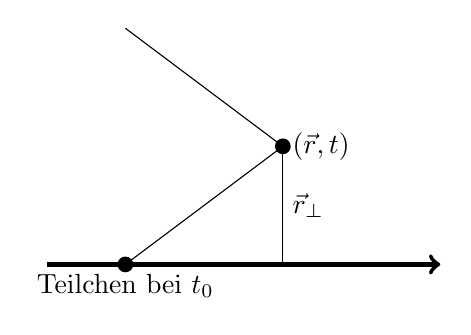
\begin{tikzpicture}
			\draw[ultra thick,->] (0,0)--(5,0);
			\fill (1,0) circle(0.1cm) node[below]{Teilchen bei $t_0$};
			\fill (3,1.5) circle(0.1cm) node[right]{$(\vec{r},t)$};
			\draw (3,0)--node[right]{$\vec{r}_\perp$}(3,1.5);
			\draw (1,0)--(3,1.5);
			\draw (1,3)--(3,1.5);
			\end{tikzpicture}
		}
	}
	\caption{Bahn}
\end{wrapfigure}
Die Bahn sei gegeben durch
\begin{equation*}
\vec{R}(t')=\begin{pmatrix}
\beta ct' \\ 0 \\ 0
\end{pmatrix}
\end{equation*}
und die Potentiale wie in Kapitel 13.5. Wir betrachten das Feld zum Zeitpunkt $t=0$. Da die Ladung unbeschleunigt ist, ist auch der Anteil $\vec{E}_a$ gleich Null. Das übrige Feld ist dann
\begin{equation*}
\vec{E}_v = \frac{Q}{4\pi\epsilon_0}\frac{\gamma\vec{r}}{(\gamma^2x^2+r_\perp^2)^\frac{3}{2}}.
\end{equation*}
Das ist offensichtlich trotz Punktladung nicht kugelsymmetriscch, sondern abhängig von $\gamma$ in $x$-Richtung gestaucht.
\newpage
\textbf{ii) \quad Energieabstrahlung}\\

Da sich die beiden Felder $\vec{E}$ und $\vec{B}$ abhängig von der Beschleunigung in zwei verschiedene Anteile aufteilen, trifft das auch für die Energiestromdichte zu.
\begin{align*}
\vec{S}_P &= \frac{\vec{E}\times\vec{B}}{\mu_0} = \frac{1}{\mu_0}(\underbrace{\vec{E}_v}_{\sim L^{-2}}+\underbrace{\vec{E}_a}_{\sim L^{-1}}) \ \times \ (\vec{B}_v+\vec{B}_a) \\
&=\underbrace{\frac{1}{\mu_0}\vec{E}_a\times\vec{B}_a}_{\text{Abstrahlung ins Unendliche}} + \underbrace{o\left(\frac{1}{L^3},\frac{1}{L^3}\right)}_{\text{Abstrahlung ins Endliche}}.
\end{align*}
Der vordere Abstrahlungsterm ist der Entscheidende, da der hintere Term sehr schnell abklingen wird.
\begin{equation*}
\vec{S}_a = \frac{1}{\mu_0}\left(\vec{E}_a+\vec{B}_a\right) = 
\frac{1}{\mu_0c}\left[\vec{e}_\text{\textit{L}}\vec{E}_a^2\right]_{\text{ret}}
\end{equation*}
Damit lässt sich die ausschlaggebende Abstrahlung von einer Bahnkurve  formulieren.  Die im Zeitintervall $\mathrm{d}t'$ am Ort $\vec{R}(t')$ in Richtung $\mathrm{d}\Omega$ abgestrahlte Energie $\mathrm{d}E(t')$ soll bei $(\vec{r},t)$ mit
\begin{align*}
t &= t' + \frac{|\vec{r}-\vec{R}(t')|}{c} & \mathrm{d}t &= \diff{t}{t'}\mathrm{t'}
\end{align*} 
beobachtet werden. 
\begin{equation*}
\d E(t') = \diff{t}{t'}\d t'\vec{S}(\vec{r},t) \cdot\vec{e}_{\vec{r}-\vec{R}(t')}\d\Omega L^2
\end{equation*}
Das führt dann schließlich auf die Leistungsabstrahlung
\begin{equation*}
\diff{P}{\Omega} \ = \  \frac{\d E(t')}{\d t\d\Omega} \ = \ \frac{1}{\mu_0c}(L\vec{E})^2k \ = \ \frac{Q^2}{16\pi^2\epsilon_0c} \frac{1}{k^5}\left(\vec{e}_L\times\left[(\vec{e}_L-\vec{\beta})\times\dot{\vec{\beta}}\right]\right)^2_\text{ret},
\end{equation*}
die nur durch $\vec{e}_L$ und die Bahnkurve bestimmt wird. Sie ist damit unabhängig vom Beobachter, was sehr sinnvoll erscheint. \\
\newpage
\textbf{iii) \quad Nichtrelativistischer Grenzfall}\\

\begin{wrapfigure}[11]{r}[0cm]{0cm}
	\raisebox{0pt}[\dimexpr\height-1\baselineskip\relax]{
		\colorbox{hgrey}{
			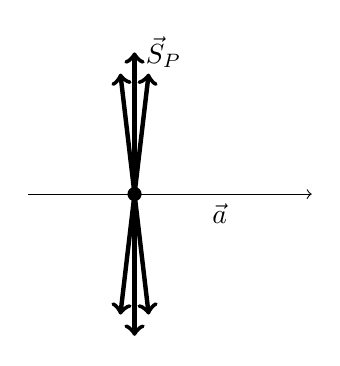
\begin{tikzpicture}[scale=.9]
			\draw[->] (0,0)--(4,0);
			\draw (2.7,0) node[below]{$\vec{a}$};
			\fill (1.5,0) circle(0.1cm);
			\draw[ultra thick,->] (1.5,0)--(1.5,2) node[right]{$\vec{S}_P$};
			\draw[ultra thick,->] (1.5,0)--(1.3,1.7);
			\draw[ultra thick,->] (1.5,0)--(1.3,-1.7);
			\draw[ultra thick,->] (1.5,0)--(1.7,1.7);
			\draw[ultra thick,->] (1.5,0)--(1.7,-1.7);
			\draw[ultra thick,->] (1.5,0)--(1.5,-2);
			\end{tikzpicture}
		}
	}
	\caption{nichtrelativistische Strahlung}
\end{wrapfigure}
Sollte $\beta \ll 1$ und damit $k\approx 1$ sein, wird die Abstrahlung
\begin{equation*}
\diff{P}{\Omega}=\frac{Q^2}{16\pi^2\epsilon_0c}|\dot{\vec{\beta}}|^2\sin^2\vartheta_a\qquad\text{mit}\quad\vartheta_a=\sphericalangle\left(\vec{e}_L,\dot{\vec{\beta}}\right)
\end{equation*}
senkrecht zur Beschleunigung $\vec{a}$ maximal. Das entspricht tatsächlich einem \textsc{Hertz}'schen Dipol.\\[2cm]
\textbf{iv) \quad Ultrarelativistischer Grenzfall}\\

Es wird $\beta\approx 1$ und 
\begin{equation*}
k=1-\dot{\vec{e}}_L\cdot\vec{\beta}\approx 1-\cos\vartheta_v\qquad\text{mit}\quad\vartheta_v=\sphericalangle\left(\vec{e}_L,\vec{\beta}\right).
\end{equation*} 
Somit ist für sehr große Geschwindigkeiten die Strahlung
\begin{align*}
\diff{P}{\Omega}&\sim \frac{1}{K^5}\left|\vec{e}_L\times\left[(\vec{e}_L - \vec{\beta})\times\dot{\vec{\beta}}\right]\right|^2\\
& \sim \frac{1}{(1-\cos\vartheta_v)}
\end{align*}
parallel zur Beschleunigung $\vec{a}$.\\[1cm]

\begin{figure}[hb]
	\centering
	\colorbox{hgrey}{
			\begin{tikzpicture}[scale=.9]
			\draw[->] (0,0)--(4,0);
			\draw (1,0) node[below]{$\vec{a}$};
			\fill (1.5,0) circle(0.1cm);
			\draw[ultra thick,->] (1.5,0)--(3.5,0) node[below right]{$\vec{S}_P$};
			\draw[ultra thick,->] (1.5,0)--(3.2,0.3);
			\draw[ultra thick,->] (1.5,0)--(3.2,-0.3);
			\draw[color=hgrey] (0,2) node{a};
			\draw[color=hgrey] (0,-2) node{a};
			\end{tikzpicture}
	}
	\caption{relativistische Strahlung}
\end{figure}